% =============================================================================
% Dictionary Diagram Style Exploration — v2 (book-quality)
% Six distinct approaches for presenting PDF signature dictionaries
% =============================================================================
\documentclass[11pt,a4paper]{article}

\usepackage{fontspec}
\setmainfont{Noto Serif}[
    BoldFont={Noto Serif Bold},
    ItalicFont={Noto Serif Italic},
    BoldItalicFont={Noto Serif Bold Italic}
]
\setsansfont{Noto Sans}[
    BoldFont={Noto Sans Bold},
    ItalicFont={Noto Sans Italic}
]
\setmonofont{DejaVu Sans Mono}[Scale=0.82]

\usepackage[inner=0.7in,outer=0.6in,top=0.65in,bottom=0.65in]{geometry}
\usepackage{xcolor}
\usepackage{tikz}
\usetikzlibrary{
    arrows.meta, positioning, calc, decorations.pathreplacing,
    shapes.geometric, shapes.multipart, fit, backgrounds,
    chains, matrix, shadows.blur
}
\usepackage{tcolorbox}
\tcbuselibrary{breakable,skins}
\usepackage{hyperref}
\hypersetup{colorlinks=true,linkcolor=linkblue}
\usepackage{microtype}
\usepackage{setspace}
\setstretch{1.06}
\usepackage{enumitem}
\setlist{noitemsep,topsep=2pt}

% =============================================================================
% Color palette
% =============================================================================
\definecolor{accent}{HTML}{1a3a5c}
\definecolor{linkblue}{HTML}{1a73e8}

% Dark code theme
\definecolor{codebg}{HTML}{1e1e2e}
\definecolor{codetext}{HTML}{cdd6f4}
\definecolor{keycolor}{HTML}{89b4fa}
\definecolor{valcolor}{HTML}{a6e3a1}
\definecolor{strcolor}{HTML}{f9e2af}
\definecolor{commentcolor}{HTML}{6c7086}
\definecolor{delimcolor}{HTML}{f38ba8}

% Annotation / callout
\definecolor{annobg}{HTML}{f0f4f8}
\definecolor{annoframe}{HTML}{94a3b8}

% Status badges
\definecolor{reqred}{HTML}{dc2626}
\definecolor{optgreen}{HTML}{16a34a}
\definecolor{condpurple}{HTML}{7c3aed}

% Grouping pastels
\definecolor{grpIdentity}{HTML}{dbeafe}
\definecolor{grpIdentityDark}{HTML}{3b82f6}
\definecolor{grpCrypto}{HTML}{d1fae5}
\definecolor{grpCryptoDark}{HTML}{059669}
\definecolor{grpMeta}{HTML}{fef3c7}
\definecolor{grpMetaDark}{HTML}{d97706}
\definecolor{grpIntegrity}{HTML}{fce7f3}
\definecolor{grpIntegrityDark}{HTML}{db2777}
\definecolor{grpBuild}{HTML}{ede9fe}
\definecolor{grpBuildDark}{HTML}{7c3aed}

% Blueprint
\definecolor{bpbg}{HTML}{f8fafc}
\definecolor{bpgrid}{HTML}{e2e8f0}
\definecolor{bpline}{HTML}{334155}

\pagestyle{empty}

\begin{document}

% =============================================================================
% STYLE 1: Blueprint / Technical Drawing
% =============================================================================
\begin{center}
{\LARGE\bfseries\sffamily\color{accent} Style 1 — Technical Blueprint}\\[3pt]
{\small\sffamily Structured like an engineering drawing. Grid background, precise connector lines, labeled zones.}
\end{center}
\vspace{0.5em}

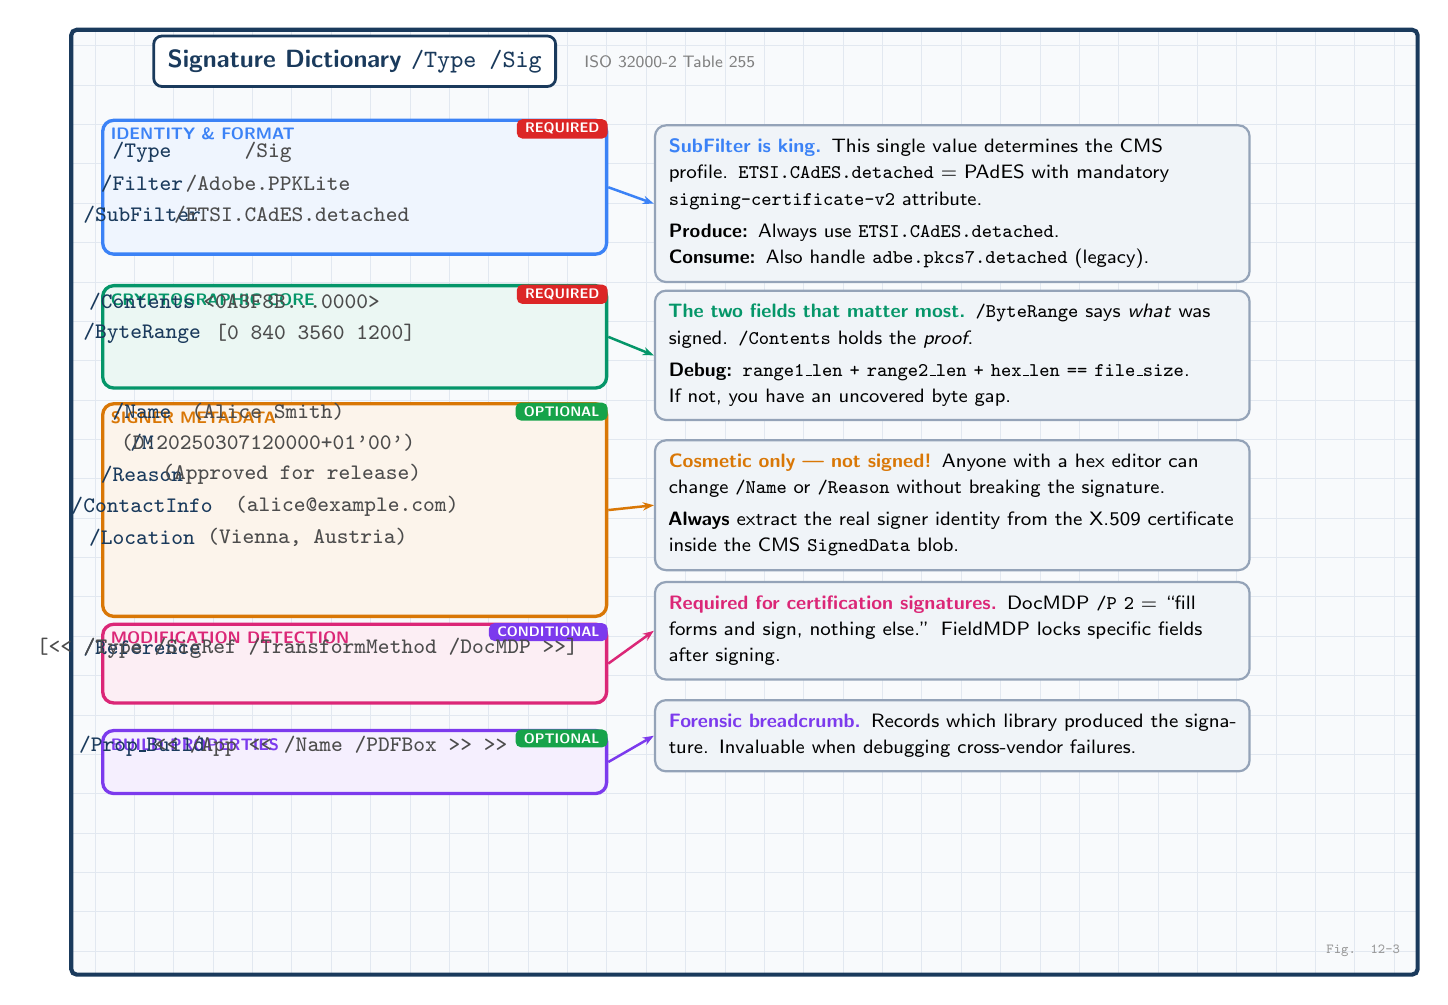
\begin{tikzpicture}[remember picture,
    every node/.style={font=\sffamily},
    zone/.style={
        rectangle, rounded corners=4pt, draw=#1, line width=1.2pt,
        fill=#1!8, inner sep=6pt,
    },
    entry/.style={
        anchor=west, font=\fontsize{8}{10}\selectfont\ttfamily,
        inner sep=0pt,
    },
    keyfont/.style={font=\fontsize{8}{10}\selectfont\ttfamily\bfseries, text=accent},
    valfont/.style={font=\fontsize{8}{10}\selectfont\ttfamily, text=black!70},
    badge/.style={
        rectangle, rounded corners=2pt, font=\fontsize{5.5}{6.5}\selectfont\bfseries\sffamily,
        text=white, inner xsep=3pt, inner ysep=1.5pt,
    },
    callout/.style={
        rectangle, rounded corners=4pt, draw=annoframe, line width=0.8pt,
        fill=annobg, text width=7.2cm, inner sep=5pt, anchor=north west,
        font=\fontsize{7.5}{9.5}\selectfont\sffamily,
    },
    connector/.style={
        draw=bpline, line width=0.9pt, -{Stealth[length=4pt, width=3pt]},
    },
    dashed connector/.style={
        draw=bpline, line width=0.7pt, dashed, -{Stealth[length=3.5pt, width=2.5pt]},
    },
]

% Grid background
\begin{scope}[on background layer]
    \fill[bpbg] (-0.3, 1.2) rectangle (16.8, -10.8);
    \foreach \x in {0,0.5,...,16.5} {
        \draw[bpgrid, line width=0.15pt] (\x, 1.2) -- (\x, -10.8);
    }
    \foreach \y in {1.0,0.5,...,-10.5} {
        \draw[bpgrid, line width=0.15pt] (-0.3, \y) -- (16.8, \y);
    }
\end{scope}

% Title cartouche
\node[rectangle, rounded corners=3pt, draw=accent, line width=1pt, fill=white,
      inner sep=5pt, font=\fontsize{9}{11}\selectfont\sffamily\bfseries, text=accent]
      (title) at (3.3, 0.8) {Signature Dictionary \texttt{/Type /Sig}};
\node[font=\fontsize{6.5}{7.5}\selectfont\sffamily\color{black!50}, anchor=west]
      at (title.east) {\quad ISO 32000-2 Table 255};

% ── Zone A: Identity & Format ───────────────────────────────────────────
\node[zone=grpIdentityDark, minimum width=6.4cm, minimum height=1.7cm]
      (zA) at (3.3, -0.8) {};
\node[font=\fontsize{6.5}{7.5}\selectfont\bfseries\sffamily, text=grpIdentityDark,
      anchor=north west] at (zA.north west) {IDENTITY \& FORMAT};
\node[badge, fill=reqred, anchor=north east] at (zA.north east) {REQUIRED};

\node[keyfont] at (0.6, -0.35) {/Type};
\node[valfont] at (2.2, -0.35) {/Sig};
\node[keyfont] at (0.6, -0.75) {/Filter};
\node[valfont] at (2.2, -0.75) {/Adobe.PPKLite};
\node[keyfont] at (0.6, -1.15) {/SubFilter};
\node[valfont] at (2.5, -1.15) {/ETSI.CAdES.detached};

% ── Zone B: Cryptographic Core ──────────────────────────────────────────
\node[zone=grpCryptoDark, minimum width=6.4cm, minimum height=1.3cm]
      (zB) at (3.3, -2.7) {};
\node[font=\fontsize{6.5}{7.5}\selectfont\bfseries\sffamily, text=grpCryptoDark,
      anchor=north west] at (zB.north west) {CRYPTOGRAPHIC CORE};
\node[badge, fill=reqred, anchor=north east] at (zB.north east) {REQUIRED};

\node[keyfont] at (0.6, -2.25) {/Contents};
\node[valfont] at (2.5, -2.25) {<0A3F8B...0000>};
\node[keyfont] at (0.6, -2.65) {/ByteRange};
\node[valfont] at (2.8, -2.65) {[0 840 3560 1200]};

% ── Zone C: Signer Metadata ────────────────────────────────────────────
\node[zone=grpMetaDark, minimum width=6.4cm, minimum height=2.7cm]
      (zC) at (3.3, -4.9) {};
\node[font=\fontsize{6.5}{7.5}\selectfont\bfseries\sffamily, text=grpMetaDark,
      anchor=north west] at (zC.north west) {SIGNER METADATA};
\node[badge, fill=optgreen, anchor=north east] at (zC.north east) {OPTIONAL};

\node[keyfont] at (0.6, -3.65) {/Name};
\node[valfont] at (2.2, -3.65) {(Alice Smith)};
\node[keyfont] at (0.6, -4.05) {/M};
\node[valfont] at (2.2, -4.05) {(D:20250307120000+01'00')};
\node[keyfont] at (0.6, -4.45) {/Reason};
\node[valfont] at (2.5, -4.45) {(Approved for release)};
\node[keyfont] at (0.6, -4.85) {/ContactInfo};
\node[valfont] at (3.2, -4.85) {(alice@example.com)};
\node[keyfont] at (0.6, -5.25) {/Location};
\node[valfont] at (2.7, -5.25) {(Vienna, Austria)};

% ── Zone D: Integrity ──────────────────────────────────────────────────
\node[zone=grpIntegrityDark, minimum width=6.4cm, minimum height=1.0cm]
      (zD) at (3.3, -6.85) {};
\node[font=\fontsize{6.5}{7.5}\selectfont\bfseries\sffamily, text=grpIntegrityDark,
      anchor=north west] at (zD.north west) {MODIFICATION DETECTION};
\node[badge, fill=condpurple, anchor=north east] at (zD.north east) {CONDITIONAL};

\node[keyfont] at (0.6, -6.65) {/Reference};
\node[valfont] at (2.7, -6.65) {[<< /Type /SigRef /TransformMethod /DocMDP >>]};

% ── Zone E: Build ──────────────────────────────────────────────────────
\node[zone=grpBuildDark, minimum width=6.4cm, minimum height=0.8cm]
      (zE) at (3.3, -8.1) {};
\node[font=\fontsize{6.5}{7.5}\selectfont\bfseries\sffamily, text=grpBuildDark,
      anchor=north west] at (zE.north west) {BUILD PROPERTIES};
\node[badge, fill=optgreen, anchor=north east] at (zE.north east) {OPTIONAL};

\node[keyfont] at (0.6, -7.9) {/Prop\_Build};
\node[valfont] at (3.0, -7.9) {<< /App << /Name /PDFBox >> >>};

% ── Callout annotations on the right ──────────────────────────────────
\node[callout] (cA) at (7.1, 0.0) {
    \textbf{\color{grpIdentityDark}SubFilter is king.}
    This single value determines the CMS profile.
    \texttt{ETSI.CAdES.detached} = PAdES with mandatory
    \texttt{signing-certificate-v2} attribute.\\[2pt]
    \textbf{Produce:} Always use \texttt{ETSI.CAdES.detached}.\\
    \textbf{Consume:} Also handle \texttt{adbe.pkcs7.detached} (legacy).
};

\node[callout] (cB) at (7.1, -2.1) {
    \textbf{\color{grpCryptoDark}The two fields that matter most.}
    \texttt{/ByteRange} says \emph{what} was signed.
    \texttt{/Contents} holds the \emph{proof}.\\[2pt]
    \textbf{Debug:} \texttt{range1\_len + range2\_len + hex\_len == file\_size}.\\
    If not, you have an uncovered byte gap.
};

\node[callout] (cC) at (7.1, -4.0) {
    \textbf{\color{grpMetaDark}Cosmetic only --- not signed!}
    Anyone with a hex editor can change \texttt{/Name} or \texttt{/Reason}
    without breaking the signature.\\[2pt]
    \textbf{Always} extract the real signer identity from the X.509
    certificate inside the CMS \texttt{SignedData} blob.
};

\node[callout] (cD) at (7.1, -5.8) {
    \textbf{\color{grpIntegrityDark}Required for certification signatures.}
    DocMDP \texttt{/P 2} = ``fill forms and sign, nothing else.''
    FieldMDP locks specific fields after signing.
};

\node[callout] (cE) at (7.1, -7.3) {
    \textbf{\color{grpBuildDark}Forensic breadcrumb.}
    Records which library produced the signature.
    Invaluable when debugging cross-vendor failures.
};

% ── Connector arrows ──────────────────────────────────────────────────
\draw[connector, color=grpIdentityDark] (zA.east) -- (cA.west);
\draw[connector, color=grpCryptoDark]   (zB.east) -- (cB.west);
\draw[connector, color=grpMetaDark]     (zC.east) -- (cC.west);
\draw[connector, color=grpIntegrityDark](zD.east) -- (cD.west);
\draw[connector, color=grpBuildDark]    (zE.east) -- (cE.west);

% ── Outer frame ──────────────────────────────────────────────────────
\begin{scope}[on background layer]
    \draw[accent, line width=1.5pt, rounded corners=2pt]
        (-0.3, 1.2) rectangle (16.8, -10.8);
    \node[font=\fontsize{5.5}{6.5}\selectfont\ttfamily\color{black!40},
          anchor=south east] at (16.7, -10.7) {Fig. 12-3};
\end{scope}

\end{tikzpicture}

\vfill\clearpage

% =============================================================================
% STYLE 2: Dark Terminal / Hex Dump
% =============================================================================
\begin{center}
{\LARGE\bfseries\sffamily\color{accent} Style 2 — Dark Terminal with Inline Annotations}\\[3pt]
{\small\sffamily Looks like a hex editor or terminal dump. Annotations are inline, not in separate boxes.}
\end{center}
\vspace{0.5em}

\begin{tikzpicture}[remember picture,
    every node/.style={anchor=west},
    line/.style={font=\fontsize{8}{11.5}\selectfont\ttfamily, text=codetext},
    k/.style={font=\fontsize{8}{11.5}\selectfont\ttfamily\bfseries, text=keycolor},
    v/.style={font=\fontsize{8}{11.5}\selectfont\ttfamily, text=valcolor},
    s/.style={font=\fontsize{8}{11.5}\selectfont\ttfamily, text=strcolor},
    d/.style={font=\fontsize{8}{11.5}\selectfont\ttfamily, text=delimcolor},
    cm/.style={font=\fontsize{7}{9.5}\selectfont\sffamily\itshape, text=commentcolor},
    anno/.style={font=\fontsize{7}{9}\selectfont\sffamily, text=white!85,
                 anchor=west, text width=6.5cm},
    sep/.style={draw=commentcolor!30, line width=0.3pt},
    groupbox/.style={
        rectangle, rounded corners=2pt, draw=#1, line width=0.8pt,
        fill=#1!15, inner sep=3pt,
    },
]

\def\lh{0.55}  % line height
\def\codeX{0.5}
\def\annoX{9.8}
\def\sepX{9.3}

% Dark background
\fill[codebg, rounded corners=5pt] (-0.2, 0.6) rectangle (16.6, -12.2);

% ── Header ─────────────────────────────────────────────────────────────
\node[font=\fontsize{7}{8}\selectfont\sffamily\bfseries, text=commentcolor,
      anchor=west] at (\codeX, 0.3)
      {SIGNATURE DICTIONARY \textnormal{--- ISO 32000-2 \S12.8.1, Table 255}};
\draw[commentcolor!40, line width=0.5pt] (0.2, 0.05) -- (16.4, 0.05);

% ── Opening delimiter ──────────────────────────────────────────────────
\node[d] (l0) at (\codeX, -0.3) {<<};

% ── Identity group ─────────────────────────────────────────────────────
\node[k] at (\codeX+0.3, -1*\lh-0.3)  {/Type};
\node[v] at (\codeX+2.0, -1*\lh-0.3)  {/Sig};

\node[k] at (\codeX+0.3, -2*\lh-0.3)  {/Filter};
\node[v] at (\codeX+2.5, -2*\lh-0.3)  {/Adobe.PPKLite};

\node[k] at (\codeX+0.3, -3*\lh-0.3)  {/SubFilter};
\node[v] at (\codeX+3.0, -3*\lh-0.3)  {/ETSI.CAdES.detached};

% Identity group box
\begin{scope}[on background layer]
    \node[groupbox=grpIdentityDark!60, fit={(\codeX+0.1, -0.5)(\codeX+8.5, -3*\lh-0.55)}] {};
\end{scope}

% Separator + annotation
\draw[sep] (\sepX, -0.4) -- (\sepX, -3*\lh-0.55);
\node[anno] at (\annoX, -0.6) {
    \textbf{\textcolor{grpIdentityDark!70}{Identity \& Format}}
    \hfill\textcolor{reqred!80}{\scriptsize\bfseries REQUIRED}\\[1pt]
    \texttt{/SubFilter} determines the CMS profile.
    Use \texttt{ETSI.CAdES.detached} for PAdES.
    Legacy: \texttt{adbe.pkcs7.detached}.
};

% ── Crypto group ───────────────────────────────────────────────────────
\def\cryptoY{-2.5}
\node[k] at (\codeX+0.3, \cryptoY-1*\lh)  {/Contents};
\node[s] at (\codeX+2.8, \cryptoY-1*\lh)  {<0A3F8B...0000>};

\node[k] at (\codeX+0.3, \cryptoY-2*\lh)  {/ByteRange};
\node[v] at (\codeX+3.0, \cryptoY-2*\lh)  {[0 840 3560 1200]};

\begin{scope}[on background layer]
    \node[groupbox=grpCryptoDark!60,
          fit={(\codeX+0.1, \cryptoY-0.35)(\codeX+8.5, \cryptoY-2*\lh-0.25)}] {};
\end{scope}

\draw[sep] (\sepX, \cryptoY-0.35) -- (\sepX, \cryptoY-2*\lh-0.25);
\node[anno] at (\annoX, \cryptoY-0.5) {
    \textbf{\textcolor{grpCryptoDark!70}{Cryptographic Core}}
    \hfill\textcolor{reqred!80}{\scriptsize\bfseries REQUIRED}\\[1pt]
    \texttt{/ByteRange} = what was signed.\\
    \texttt{/Contents} = the CMS proof.\\[1pt]
    \textbf{Check:} \texttt{sum(ranges) + hex\_len == file\_size}
};

% ── Metadata group ─────────────────────────────────────────────────────
\def\metaY{-4.6}
\node[k] at (\codeX+0.3, \metaY-1*\lh)   {/Name};
\node[s] at (\codeX+2.0, \metaY-1*\lh)   {(Alice Smith)};

\node[k] at (\codeX+0.3, \metaY-2*\lh)   {/M};
\node[s] at (\codeX+1.5, \metaY-2*\lh)   {(D:20250307120000+01'00')};

\node[k] at (\codeX+0.3, \metaY-3*\lh)   {/Reason};
\node[s] at (\codeX+2.5, \metaY-3*\lh)   {(Approved for release)};

\node[k] at (\codeX+0.3, \metaY-4*\lh)   {/ContactInfo};
\node[s] at (\codeX+3.5, \metaY-4*\lh)   {(alice@example.com)};

\node[k] at (\codeX+0.3, \metaY-5*\lh)   {/Location};
\node[s] at (\codeX+2.8, \metaY-5*\lh)   {(Vienna, Austria)};

\begin{scope}[on background layer]
    \node[groupbox=grpMetaDark!60,
          fit={(\codeX+0.1, \metaY-0.35)(\codeX+8.5, \metaY-5*\lh-0.25)}] {};
\end{scope}

\draw[sep] (\sepX, \metaY-0.35) -- (\sepX, \metaY-5*\lh-0.25);
\node[anno] at (\annoX, \metaY-0.5) {
    \textbf{\textcolor{grpMetaDark!70}{Signer Metadata}}
    \hfill\textcolor{optgreen!80}{\scriptsize\bfseries OPTIONAL}\\[1pt]
    \textbf{Not signed!} Anyone can change these
    with a hex editor. The real identity lives
    in the X.509 cert inside \texttt{/Contents}.
};

% ── Integrity group ────────────────────────────────────────────────────
\def\intY{-8.2}
\node[k] at (\codeX+0.3, \intY-1*\lh)    {/Reference};
\node[v] at (\codeX+2.8, \intY-1*\lh)    {[<<};
\node[k] at (\codeX+0.8, \intY-2*\lh)    {/Type};
\node[v] at (\codeX+2.2, \intY-2*\lh)    {/SigRef};
\node[k] at (\codeX+0.8, \intY-3*\lh)    {/TransformMethod};
\node[v] at (\codeX+4.2, \intY-3*\lh)    {/DocMDP};
\node[k] at (\codeX+0.8, \intY-4*\lh)    {/TransformParams};
\node[v] at (\codeX+4.5, \intY-4*\lh)    {<< /P 2 >>};
\node[v] at (\codeX+0.3, \intY-5*\lh)    {>>]};

\begin{scope}[on background layer]
    \node[groupbox=grpIntegrityDark!60,
          fit={(\codeX+0.1, \intY-0.35)(\codeX+8.5, \intY-5*\lh-0.15)}] {};
\end{scope}

\draw[sep] (\sepX, \intY-0.35) -- (\sepX, \intY-5*\lh-0.15);
\node[anno] at (\annoX, \intY-0.5) {
    \textbf{\textcolor{grpIntegrityDark!70}{Modification Detection}}
    \hfill\textcolor{condpurple!80}{\scriptsize\bfseries CONDITIONAL}\\[1pt]
    Required for certification signatures.\\
    \texttt{/P 2} = fill forms + sign only.\\
    \texttt{/P 3} = annotations also allowed.
};

% ── Build group ────────────────────────────────────────────────────────
\def\buildY{-11.3}
\node[k] at (\codeX+0.3, \buildY)         {/Prop\_Build};
\node[v] at (\codeX+3.3, \buildY)         {<< /App << /Name /PDFBox >> >>};

\begin{scope}[on background layer]
    \node[groupbox=grpBuildDark!60,
          fit={(\codeX+0.1, \buildY+0.2)(\codeX+8.5, \buildY-0.3)}] {};
\end{scope}

\draw[sep] (\sepX, \buildY+0.2) -- (\sepX, \buildY-0.3);
\node[anno] at (\annoX, \buildY+0.1) {
    \textbf{\textcolor{grpBuildDark!70}{Build Properties}}
    \hfill\textcolor{optgreen!80}{\scriptsize\bfseries OPTIONAL}\\[1pt]
    Which library created the signature.
};

% ── Closing delimiter ─────────────────────────────────────────────────
\node[d] at (\codeX, \buildY-0.6) {>>};

\end{tikzpicture}

\vfill\clearpage

% =============================================================================
% STYLE 3: Exploded Diagram with Zoom Insets
% =============================================================================
\begin{center}
{\LARGE\bfseries\sffamily\color{accent} Style 3 — Exploded View with Zoom Insets}\\[3pt]
{\small\sffamily Central compact dictionary. Key entries ``explode'' outward to detailed inset panels.}
\end{center}
\vspace{0.5em}

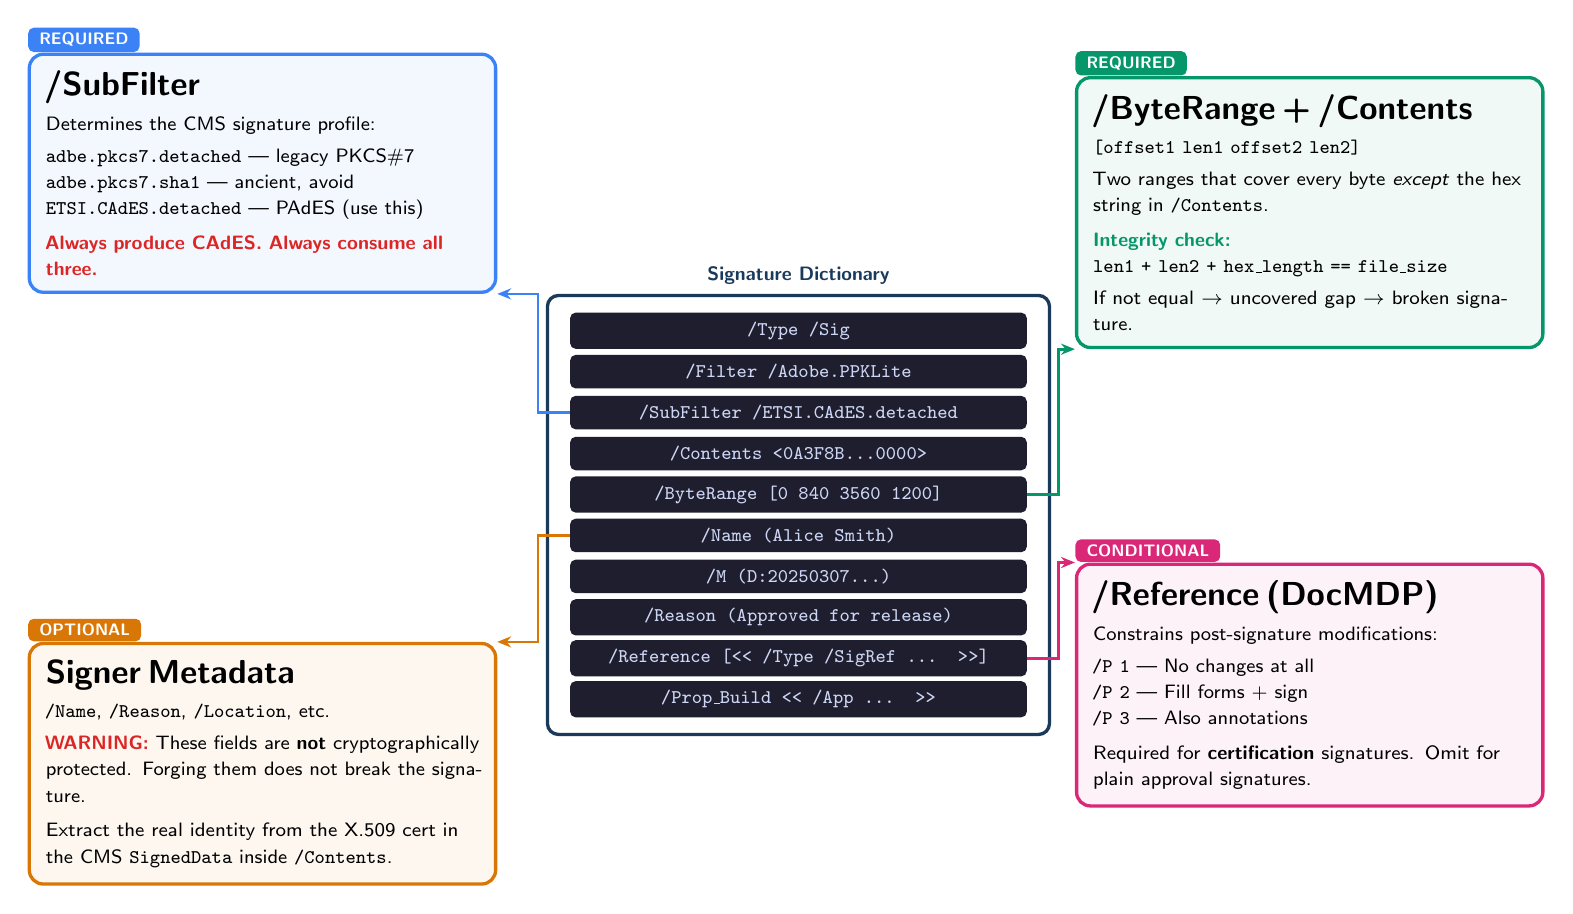
\begin{tikzpicture}[remember picture,
    every node/.style={font=\sffamily},
    dictentry/.style={
        rectangle, rounded corners=2pt,
        fill=codebg, text=codetext,
        font=\fontsize{7.5}{9.5}\selectfont\ttfamily,
        minimum width=5.8cm, minimum height=0.4cm,
        anchor=west, inner xsep=5pt,
    },
    inset/.style={
        rectangle, rounded corners=5pt,
        draw=#1, line width=1.2pt,
        fill=#1!6, inner sep=6pt,
        text width=5.5cm, anchor=center,
        font=\fontsize{7.5}{9.5}\selectfont\sffamily,
    },
    insetlabel/.style={
        rectangle, rounded corners=2pt,
        fill=#1, text=white,
        font=\fontsize{6.5}{7.5}\selectfont\bfseries\sffamily,
        inner xsep=4pt, inner ysep=2pt,
    },
    zoom/.style={
        draw=#1, line width=1pt, -{Stealth[length=5pt, width=4pt]},
    },
]

% ── Central dictionary stack ───────────────────────────────────────────
\def\startY{0}
\def\entryH{0.52}

\node[dictentry] (e1)  at (5.1, \startY)             {/Type /Sig};
\node[dictentry] (e2)  at (5.1, \startY-1*\entryH)   {/Filter /Adobe.PPKLite};
\node[dictentry] (e3)  at (5.1, \startY-2*\entryH)   {/SubFilter /ETSI.CAdES.detached};
\node[dictentry] (e4)  at (5.1, \startY-3*\entryH)   {/Contents <0A3F8B...0000>};
\node[dictentry] (e5)  at (5.1, \startY-4*\entryH)   {/ByteRange [0 840 3560 1200]};
\node[dictentry] (e6)  at (5.1, \startY-5*\entryH)   {/Name (Alice Smith)};
\node[dictentry] (e7)  at (5.1, \startY-6*\entryH)   {/M (D:20250307...)};
\node[dictentry] (e8)  at (5.1, \startY-7*\entryH)   {/Reason (Approved for release)};
\node[dictentry] (e9)  at (5.1, \startY-8*\entryH)   {/Reference [<< /Type /SigRef ... >>]};
\node[dictentry] (e10) at (5.1, \startY-9*\entryH)   {/Prop\_Build << /App ... >>};

% Frame around dict
\begin{scope}[on background layer]
    \node[fit=(e1)(e10), inner xsep=8pt, inner ysep=6pt,
          draw=accent, line width=1.2pt, rounded corners=4pt, fill=white] (dictframe) {};
\end{scope}
\node[font=\fontsize{7}{8}\selectfont\bfseries\sffamily\color{accent},
      anchor=south] at (dictframe.north) {Signature Dictionary};

% ── Inset: SubFilter (top-left) ───────────────────────────────────────
\node[inset=grpIdentityDark] (iA) at (1.2, 2.0) {
    \textbf{\large /SubFilter}\\[3pt]
    Determines the CMS signature profile:\\[2pt]
    \texttt{adbe.pkcs7.detached} --- legacy PKCS\#7\\
    \texttt{adbe.pkcs7.sha1} --- ancient, avoid\\
    \texttt{ETSI.CAdES.detached} --- PAdES (use this)\\[3pt]
    \textcolor{reqred}{\bfseries Always produce CAdES. Always consume all three.}
};
\node[insetlabel=grpIdentityDark, anchor=south west] at (iA.north west) {REQUIRED};
\draw[zoom=grpIdentityDark] (e3.west) -- ++(-0.4,0) |- (iA.south east);

% ── Inset: ByteRange (top-right) ──────────────────────────────────────
\node[inset=grpCryptoDark] (iB) at (14.5, 1.5) {
    \textbf{\large /ByteRange + /Contents}\\[3pt]
    \texttt{[offset1 len1 offset2 len2]}\\[2pt]
    Two ranges that cover every byte \emph{except}
    the hex string in \texttt{/Contents}.\\[3pt]
    \textcolor{grpCryptoDark}{\bfseries Integrity check:}\\
    \texttt{len1 + len2 + hex\_length == file\_size}\\[2pt]
    If not equal \(\rightarrow\) uncovered gap \(\rightarrow\) broken signature.
};
\node[insetlabel=grpCryptoDark, anchor=south west] at (iB.north west) {REQUIRED};
\draw[zoom=grpCryptoDark] (e5.east) -- ++(0.4,0) |- (iB.south west);

% ── Inset: Metadata (bottom-left) ─────────────────────────────────────
\node[inset=grpMetaDark] (iC) at (1.2, -5.5) {
    \textbf{\large Signer Metadata}\\[3pt]
    \texttt{/Name}, \texttt{/Reason}, \texttt{/Location}, etc.\\[2pt]
    \textcolor{reqred}{\bfseries WARNING:} These fields are \textbf{not}
    cryptographically protected. Forging them does not
    break the signature.\\[3pt]
    Extract the real identity from the X.509 cert
    in the CMS \texttt{SignedData} inside \texttt{/Contents}.
};
\node[insetlabel=grpMetaDark, anchor=south west] at (iC.north west) {OPTIONAL};
\draw[zoom=grpMetaDark] (e6.west) -- ++(-0.4,0) |- (iC.north east);

% ── Inset: Reference (bottom-right) ───────────────────────────────────
\node[inset=grpIntegrityDark] (iD) at (14.5, -4.5) {
    \textbf{\large /Reference (DocMDP)}\\[3pt]
    Constrains post-signature modifications:\\[2pt]
    \texttt{/P 1} --- No changes at all\\
    \texttt{/P 2} --- Fill forms + sign\\
    \texttt{/P 3} --- Also annotations\\[3pt]
    Required for \textbf{certification} signatures.
    Omit for plain approval signatures.
};
\node[insetlabel=grpIntegrityDark, anchor=south west] at (iD.north west) {CONDITIONAL};
\draw[zoom=grpIntegrityDark] (e9.east) -- ++(0.4,0) |- (iD.north west);

\end{tikzpicture}

\vfill\clearpage

% =============================================================================
% STYLE 4: Structured Table with Visual Hierarchy
% =============================================================================
\begin{center}
{\LARGE\bfseries\sffamily\color{accent} Style 4 — Structured Table with Row Grouping}\\[3pt]
{\small\sffamily Clean tabular layout. Color-coded group headers. Right column for notes.}
\end{center}
\vspace{0.5em}

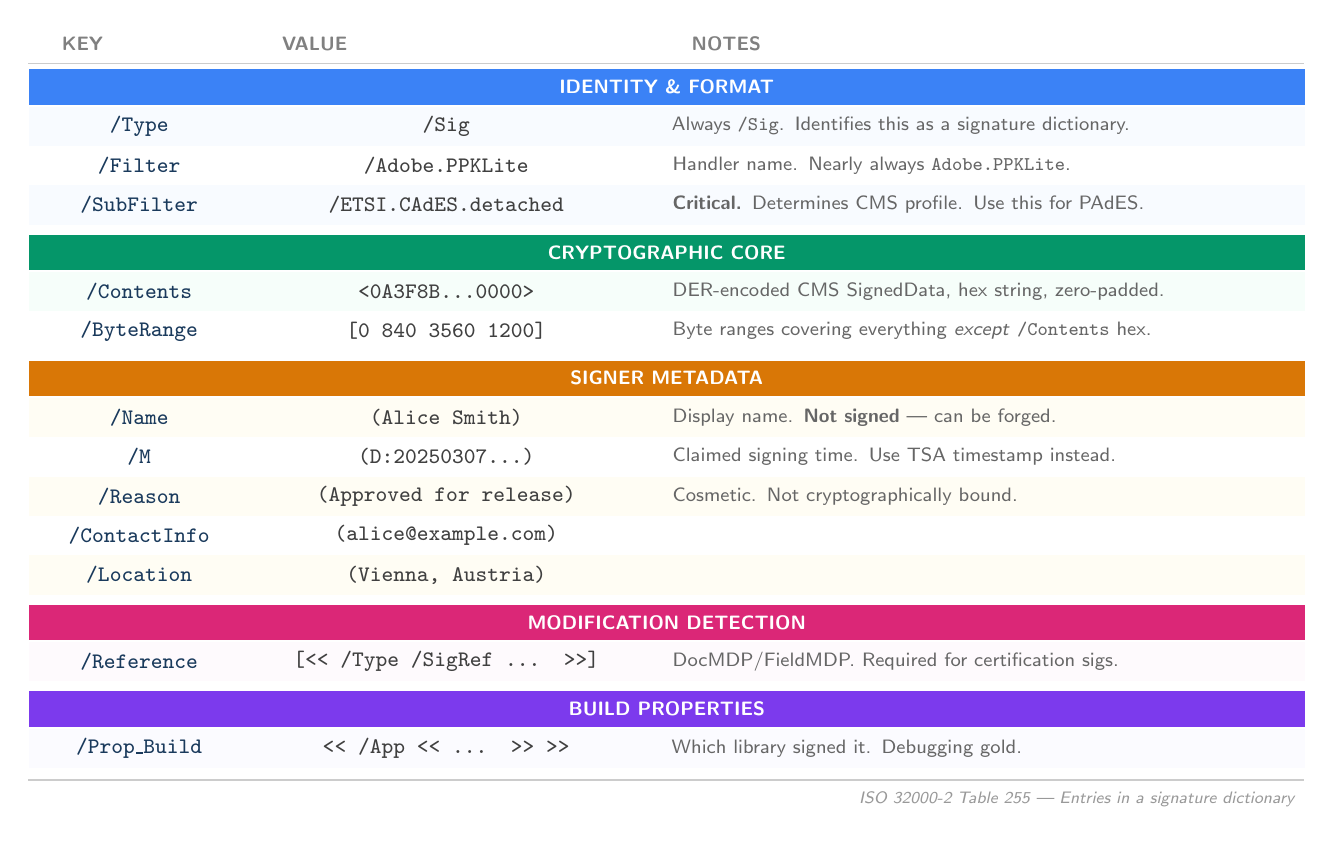
\begin{tikzpicture}[remember picture,
    every node/.style={font=\sffamily, anchor=west},
    groupheader/.style={
        rectangle, minimum width=16.2cm, minimum height=0.45cm,
        fill=#1, font=\fontsize{7.5}{9}\selectfont\bfseries\sffamily,
        text=white, inner xsep=8pt, anchor=west,
    },
    row/.style={
        rectangle, minimum width=16.2cm, minimum height=0.5cm,
        fill=#1, inner xsep=0pt, anchor=west,
    },
    keycell/.style={
        font=\fontsize{8}{10}\selectfont\ttfamily\bfseries, text=accent,
        minimum width=2.8cm, anchor=west, inner xsep=8pt,
    },
    valcell/.style={
        font=\fontsize{8}{10}\selectfont\ttfamily, text=black!75,
        minimum width=5cm, anchor=west,
    },
    notecell/.style={
        font=\fontsize{7}{9}\selectfont\sffamily, text=black!60,
        text width=7.5cm, anchor=west, inner xsep=5pt,
    },
    colheader/.style={
        font=\fontsize{7}{8}\selectfont\bfseries\sffamily\color{black!50},
        anchor=west,
    },
]

\def\rh{0.5}
\def\colK{0}
\def\colV{2.8}
\def\colN{8.0}

% Column headers
\node[colheader] at (\colK+0.3, 0.3) {KEY};
\node[colheader] at (\colV+0.3, 0.3) {VALUE};
\node[colheader] at (\colN+0.3, 0.3) {NOTES};
\draw[black!20, line width=0.5pt] (0, 0.05) -- (16.2, 0.05);

% ── Group: Identity ────────────────────────────────────────────────────
\node[groupheader=grpIdentityDark] at (0, -0.25) {IDENTITY \& FORMAT};

\node[row=grpIdentity!20]  at (0, -0.75) {};
\node[keycell]  at (\colK, -0.75) {/Type};
\node[valcell]  at (\colV, -0.75) {/Sig};
\node[notecell] at (\colN, -0.75) {Always \texttt{/Sig}. Identifies this as a signature dictionary.};

\node[row=white] at (0, -1.25) {};
\node[keycell]  at (\colK, -1.25) {/Filter};
\node[valcell]  at (\colV, -1.25) {/Adobe.PPKLite};
\node[notecell] at (\colN, -1.25) {Handler name. Nearly always \texttt{Adobe.PPKLite}.};

\node[row=grpIdentity!20] at (0, -1.75) {};
\node[keycell]  at (\colK, -1.75) {/SubFilter};
\node[valcell]  at (\colV, -1.75) {/ETSI.CAdES.detached};
\node[notecell] at (\colN, -1.75) {\textbf{Critical.} Determines CMS profile. Use this for PAdES.};

% ── Group: Crypto ──────────────────────────────────────────────────────
\node[groupheader=grpCryptoDark] at (0, -2.35) {CRYPTOGRAPHIC CORE};

\node[row=grpCrypto!20] at (0, -2.85) {};
\node[keycell]  at (\colK, -2.85) {/Contents};
\node[valcell]  at (\colV, -2.85) {<0A3F8B...0000>};
\node[notecell] at (\colN, -2.85) {DER-encoded CMS SignedData, hex string, zero-padded.};

\node[row=white] at (0, -3.35) {};
\node[keycell]  at (\colK, -3.35) {/ByteRange};
\node[valcell]  at (\colV, -3.35) {[0 840 3560 1200]};
\node[notecell] at (\colN, -3.35) {Byte ranges covering everything \emph{except} \texttt{/Contents} hex.};

% ── Group: Metadata ────────────────────────────────────────────────────
\node[groupheader=grpMetaDark] at (0, -3.95) {SIGNER METADATA};

\node[row=grpMeta!20] at (0, -4.45) {};
\node[keycell]  at (\colK, -4.45) {/Name};
\node[valcell]  at (\colV, -4.45) {(Alice Smith)};
\node[notecell] at (\colN, -4.45) {Display name. \textbf{Not signed} --- can be forged.};

\node[row=white] at (0, -4.95) {};
\node[keycell]  at (\colK, -4.95) {/M};
\node[valcell]  at (\colV, -4.95) {(D:20250307...)};
\node[notecell] at (\colN, -4.95) {Claimed signing time. Use TSA timestamp instead.};

\node[row=grpMeta!20] at (0, -5.45) {};
\node[keycell]  at (\colK, -5.45) {/Reason};
\node[valcell]  at (\colV, -5.45) {(Approved for release)};
\node[notecell] at (\colN, -5.45) {Cosmetic. Not cryptographically bound.};

\node[row=white] at (0, -5.95) {};
\node[keycell]  at (\colK, -5.95) {/ContactInfo};
\node[valcell]  at (\colV, -5.95) {(alice@example.com)};
\node[notecell] at (\colN, -5.95) {};

\node[row=grpMeta!20] at (0, -6.45) {};
\node[keycell]  at (\colK, -6.45) {/Location};
\node[valcell]  at (\colV, -6.45) {(Vienna, Austria)};
\node[notecell] at (\colN, -6.45) {};

% ── Group: Integrity ──────────────────────────────────────────────────
\node[groupheader=grpIntegrityDark] at (0, -7.05) {MODIFICATION DETECTION};

\node[row=grpIntegrity!20] at (0, -7.55) {};
\node[keycell]  at (\colK, -7.55) {/Reference};
\node[valcell]  at (\colV, -7.55) {[<< /Type /SigRef ... >>]};
\node[notecell] at (\colN, -7.55) {DocMDP/FieldMDP. Required for certification sigs.};

% ── Group: Build ──────────────────────────────────────────────────────
\node[groupheader=grpBuildDark] at (0, -8.15) {BUILD PROPERTIES};

\node[row=grpBuild!20] at (0, -8.65) {};
\node[keycell]  at (\colK, -8.65) {/Prop\_Build};
\node[valcell]  at (\colV, -8.65) {<< /App << ... >> >>};
\node[notecell] at (\colN, -8.65) {Which library signed it. Debugging gold.};

% ── Bottom border ─────────────────────────────────────────────────────
\draw[black!20, line width=0.5pt] (0, -9.05) -- (16.2, -9.05);
\node[font=\fontsize{6}{7}\selectfont\sffamily\itshape\color{black!40},
      anchor=east] at (16.2, -9.3) {ISO 32000-2 Table 255 --- Entries in a signature dictionary};

\end{tikzpicture}

\vfill\clearpage

% =============================================================================
% STYLE 5: Nested Object Graph (tree-like)
% =============================================================================
\begin{center}
{\LARGE\bfseries\sffamily\color{accent} Style 5 — Object Graph / Nested Structure}\\[3pt]
{\small\sffamily Shows the dictionary as a tree of objects with nesting depth visualized.
Reveals the structure that a flat listing hides.}
\end{center}
\vspace{0.5em}

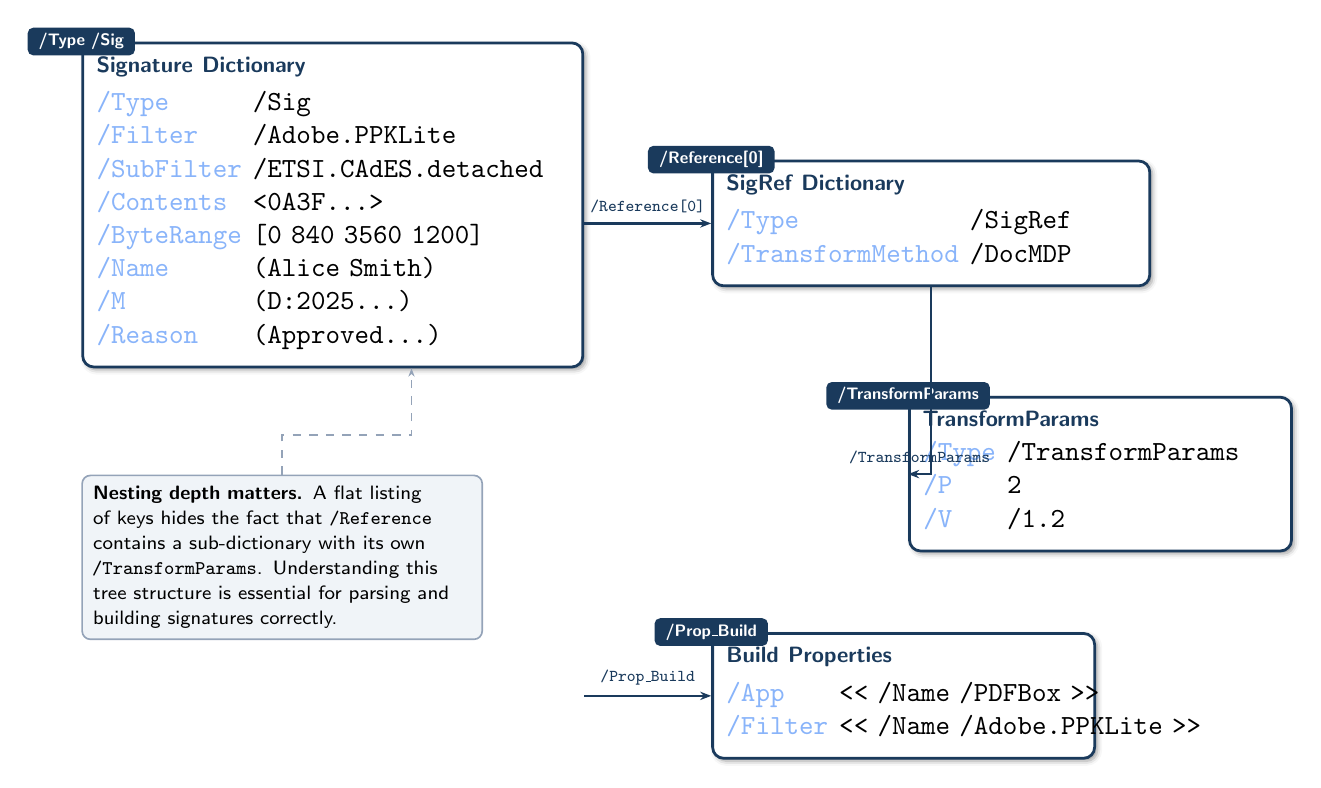
\begin{tikzpicture}[remember picture,
    every node/.style={font=\sffamily},
    dictnode/.style={
        rectangle, rounded corners=4pt,
        draw=accent, line width=1pt,
        fill=white,
        inner sep=5pt, anchor=north west,
        blur shadow={shadow blur steps=3, shadow xshift=1pt, shadow yshift=-1pt},
    },
    kvrow/.style={
        font=\fontsize{7.5}{10}\selectfont, anchor=west,
    },
    childlink/.style={
        draw=accent, line width=0.9pt,
        -{Stealth[length=4pt, width=3pt]},
    },
    nodelabel/.style={
        rectangle, rounded corners=2pt,
        fill=accent, text=white,
        font=\fontsize{6.5}{7.5}\selectfont\bfseries\sffamily,
        inner xsep=4pt, inner ysep=2pt,
    },
    note/.style={
        rectangle, rounded corners=3pt,
        fill=annobg, draw=annoframe, line width=0.6pt,
        font=\fontsize{7}{9}\selectfont\sffamily,
        text width=4.8cm, inner sep=4pt, anchor=north west,
    },
]

% ── Root: Signature Dictionary ─────────────────────────────────────────
\node[dictnode, text width=6cm] (root) at (0, 0) {
    {\bfseries\color{accent}\fontsize{8}{10}\selectfont Signature Dictionary}\\[3pt]
    \begin{tabular}{@{}l@{\hspace{4pt}}l@{}}
    \texttt{\bfseries\color{keycolor}/Type}        & \texttt{/Sig} \\
    \texttt{\bfseries\color{keycolor}/Filter}      & \texttt{/Adobe.PPKLite} \\
    \texttt{\bfseries\color{keycolor}/SubFilter}   & \texttt{/ETSI.CAdES.detached} \\
    \texttt{\bfseries\color{keycolor}/Contents}    & \texttt{<0A3F...>} \\
    \texttt{\bfseries\color{keycolor}/ByteRange}   & \texttt{[0 840 3560 1200]} \\
    \texttt{\bfseries\color{keycolor}/Name}        & \texttt{(Alice Smith)} \\
    \texttt{\bfseries\color{keycolor}/M}           & \texttt{(D:2025...)} \\
    \texttt{\bfseries\color{keycolor}/Reason}      & \texttt{(Approved...)} \\
    \end{tabular}
};
\node[nodelabel] at (root.north west) {/Type /Sig};

% ── Child: /Reference array ────────────────────────────────────────────
\node[dictnode, text width=5.2cm] (ref) at (8, -1.5) {
    {\bfseries\color{accent}\fontsize{8}{10}\selectfont SigRef Dictionary}\\[3pt]
    \begin{tabular}{@{}l@{\hspace{4pt}}l@{}}
    \texttt{\bfseries\color{keycolor}/Type}             & \texttt{/SigRef} \\
    \texttt{\bfseries\color{keycolor}/TransformMethod}  & \texttt{/DocMDP} \\
    \end{tabular}
};
\node[nodelabel] at (ref.north west) {/Reference[0]};

% ── Grandchild: /TransformParams ───────────────────────────────────────
\node[dictnode, text width=4.5cm] (params) at (10.5, -4.5) {
    {\bfseries\color{accent}\fontsize{8}{10}\selectfont TransformParams}\\[3pt]
    \begin{tabular}{@{}l@{\hspace{4pt}}l@{}}
    \texttt{\bfseries\color{keycolor}/Type} & \texttt{/TransformParams} \\
    \texttt{\bfseries\color{keycolor}/P}    & \texttt{2} \\
    \texttt{\bfseries\color{keycolor}/V}    & \texttt{/1.2} \\
    \end{tabular}
};
\node[nodelabel] at (params.north west) {/TransformParams};

% ── Child: /Prop_Build ─────────────────────────────────────────────────
\node[dictnode, text width=4.5cm] (build) at (8, -7.5) {
    {\bfseries\color{accent}\fontsize{8}{10}\selectfont Build Properties}\\[3pt]
    \begin{tabular}{@{}l@{\hspace{4pt}}l@{}}
    \texttt{\bfseries\color{keycolor}/App}  & \texttt{<< /Name /PDFBox >>} \\
    \texttt{\bfseries\color{keycolor}/Filter} & \texttt{<< /Name /Adobe.PPKLite >>} \\
    \end{tabular}
};
\node[nodelabel] at (build.north west) {/Prop\_Build};

% ── Links ──────────────────────────────────────────────────────────────
\draw[childlink] (root.east |- ref.west) -- (ref.west)
    node[midway, above, font=\fontsize{6.5}{7}\selectfont\ttfamily\color{accent}] {/Reference[0]};
\draw[childlink] (ref.south) |- (params.west)
    node[near end, above, font=\fontsize{6.5}{7}\selectfont\ttfamily\color{accent}] {/TransformParams};
\draw[childlink] (root.east |- build.west) -- (build.west)
    node[midway, above, font=\fontsize{6.5}{7}\selectfont\ttfamily\color{accent}] {/Prop\_Build};

% ── Annotation notes ──────────────────────────────────────────────────
\node[note] (n1) at (0, -5.5) {
    \textbf{Nesting depth matters.}
    A flat listing of keys hides the fact that
    \texttt{/Reference} contains a sub-dictionary
    with its own \texttt{/TransformParams}.
    Understanding this tree structure is essential
    for parsing and building signatures correctly.
};
\draw[annoframe, line width=0.6pt, dashed, -{Stealth[length=3pt]}]
    (n1.north) -- ++(0, 0.5) -| ($(root.south)+(1,0)$);

\end{tikzpicture}

\vfill\clearpage

% =============================================================================
% STYLE 6: Side-by-Side Code + Annotated Schematic
% =============================================================================
\begin{center}
{\LARGE\bfseries\sffamily\color{accent} Style 6 — Code Block + Schematic Side-by-Side}\\[3pt]
{\small\sffamily Left: raw PDF syntax (what you see in a hex editor). Right: schematic with grouping and annotations.}
\end{center}
\vspace{0.5em}

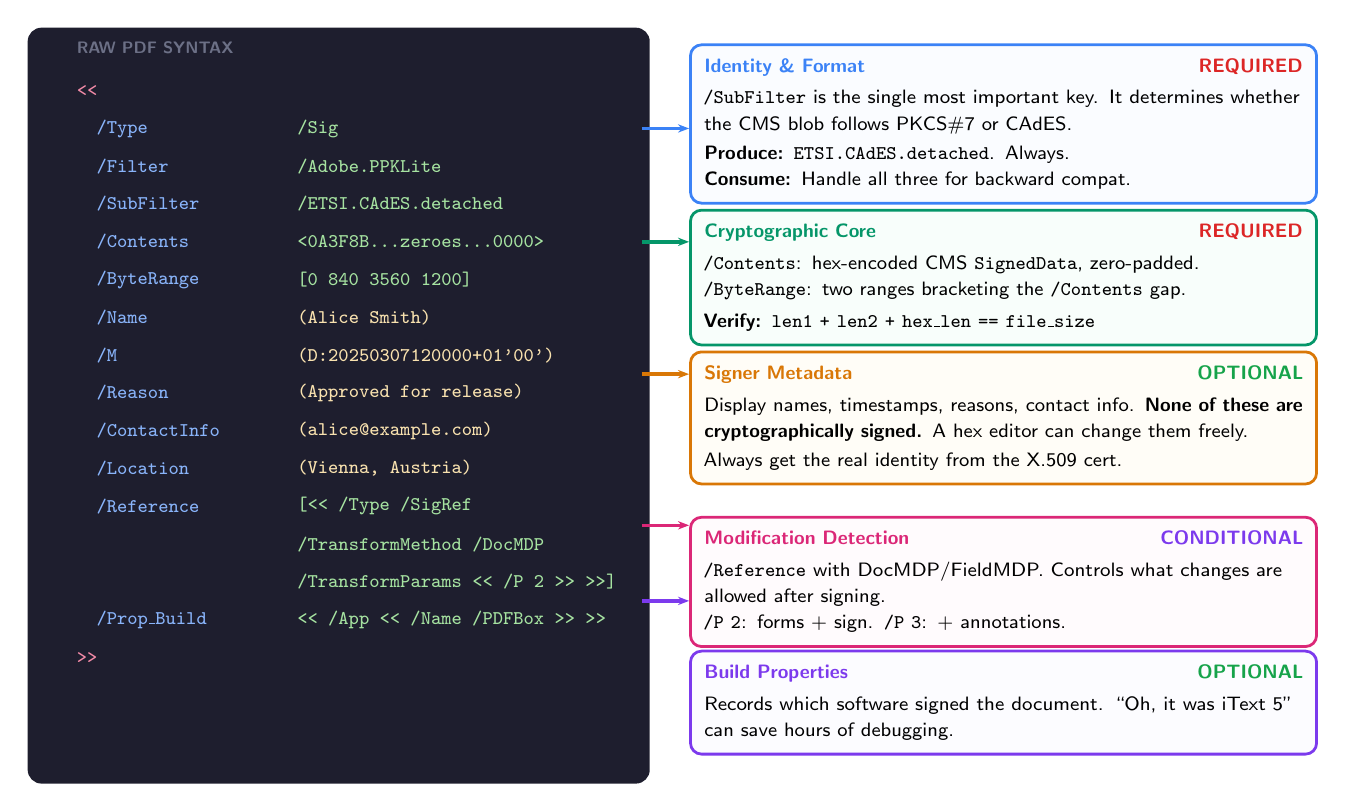
\begin{tikzpicture}[remember picture,
    every node/.style={anchor=west},
]

\def\lh{0.48}
\def\leftX{0.4}
\def\rightX{8.3}

% ── LEFT PANEL: Raw code ───────────────────────────────────────────────
\fill[codebg, rounded corners=5pt] (-0.1, 0.7) rectangle (7.8, -8.9);

\node[font=\fontsize{6.5}{7.5}\selectfont\sffamily\bfseries, text=commentcolor]
    at (\leftX, 0.45) {RAW PDF SYNTAX};

\node[font=\fontsize{7.5}{10}\selectfont\ttfamily, text=delimcolor]
    (raw0) at (\leftX, -0.1) {<<};

\foreach \i/\k/\v [count=\n from 1] in {
    1/{/Type}/{/Sig},
    2/{/Filter}/{/Adobe.PPKLite},
    3/{/SubFilter}/{/ETSI.CAdES.detached},
    4/{/Contents}/{<0A3F8B...zeroes...0000>},
    5/{/ByteRange}/{[0 840 3560 1200]},
    6/{/Name}/{(Alice Smith)},
    7/{/M}/{(D:20250307120000+01'00')},
    8/{/Reason}/{(Approved for release)},
    9/{/ContactInfo}/{(alice@example.com)},
    10/{/Location}/{(Vienna, Austria)},
    11/{/Reference}/{[<< /Type /SigRef},
    12/{}/{   /TransformMethod /DocMDP},
    13/{}/{   /TransformParams << /P 2 >> >>]},
    14/{/Prop\_Build}/{<< /App << /Name /PDFBox >> >>}%
} {
    \node[font=\fontsize{7.5}{10}\selectfont\ttfamily\bfseries, text=keycolor]
        at (\leftX+0.25, -\n*\lh-0.1) {\k};
    \ifnum\n<6
        \node[font=\fontsize{7.5}{10}\selectfont\ttfamily, text=valcolor]
            at (\leftX+2.8, -\n*\lh-0.1) {\v};
    \else\ifnum\n<11
        \node[font=\fontsize{7.5}{10}\selectfont\ttfamily, text=strcolor]
            at (\leftX+2.8, -\n*\lh-0.1) {\v};
    \else
        \node[font=\fontsize{7.5}{10}\selectfont\ttfamily, text=valcolor]
            at (\leftX+2.8, -\n*\lh-0.1) {\v};
    \fi\fi
}

\node[font=\fontsize{7.5}{10}\selectfont\ttfamily, text=delimcolor]
    at (\leftX, -15*\lh-0.1) {>>};

% ── Highlight bars on left for groups ──────────────────────────────────
\begin{scope}[on background layer]
    % Identity
    \fill[grpIdentityDark!15, rounded corners=1pt]
        (\leftX-0.1, -0.35) rectangle (7.6, -3*\lh-0.35);
    % Crypto
    \fill[grpCryptoDark!15, rounded corners=1pt]
        (\leftX-0.1, -3*\lh-0.45) rectangle (7.6, -5*\lh-0.35);
    % Metadata
    \fill[grpMetaDark!15, rounded corners=1pt]
        (\leftX-0.1, -5*\lh-0.45) rectangle (7.6, -10*\lh-0.35);
    % Integrity
    \fill[grpIntegrityDark!15, rounded corners=1pt]
        (\leftX-0.1, -10*\lh-0.45) rectangle (7.6, -13*\lh-0.35);
    % Build
    \fill[grpBuildDark!15, rounded corners=1pt]
        (\leftX-0.1, -13*\lh-0.45) rectangle (7.6, -14*\lh-0.35);
\end{scope}

% ── RIGHT PANEL: Annotated schematic ──────────────────────────────────
\def\boxW{7.6cm}

\node[rectangle, rounded corners=4pt, draw=grpIdentityDark, line width=1pt,
      fill=grpIdentity!15, text width=\boxW, inner sep=5pt, anchor=north west,
      font=\fontsize{7.5}{9.5}\selectfont\sffamily]
    (rA) at (\rightX, 0.5) {
    \textbf{\color{grpIdentityDark}Identity \& Format}
    \hfill\textcolor{reqred}{\scriptsize\bfseries REQUIRED}\\[2pt]
    \texttt{/SubFilter} is the single most important key.
    It determines whether the CMS blob follows PKCS\#7 or CAdES.\\[1pt]
    \textbf{Produce:} \texttt{ETSI.CAdES.detached}. Always.\\
    \textbf{Consume:} Handle all three for backward compat.
};

\node[rectangle, rounded corners=4pt, draw=grpCryptoDark, line width=1pt,
      fill=grpCrypto!15, text width=\boxW, inner sep=5pt, anchor=north west,
      font=\fontsize{7.5}{9.5}\selectfont\sffamily]
    (rB) at (\rightX, -1.6) {
    \textbf{\color{grpCryptoDark}Cryptographic Core}
    \hfill\textcolor{reqred}{\scriptsize\bfseries REQUIRED}\\[2pt]
    \texttt{/Contents}: hex-encoded CMS \texttt{SignedData}, zero-padded.\\
    \texttt{/ByteRange}: two ranges bracketing the \texttt{/Contents} gap.\\[2pt]
    \textbf{Verify:} \texttt{len1 + len2 + hex\_len == file\_size}
};

\node[rectangle, rounded corners=4pt, draw=grpMetaDark, line width=1pt,
      fill=grpMeta!15, text width=\boxW, inner sep=5pt, anchor=north west,
      font=\fontsize{7.5}{9.5}\selectfont\sffamily]
    (rC) at (\rightX, -3.4) {
    \textbf{\color{grpMetaDark}Signer Metadata}
    \hfill\textcolor{optgreen}{\scriptsize\bfseries OPTIONAL}\\[2pt]
    Display names, timestamps, reasons, contact info.
    \textbf{None of these are cryptographically signed.}
    A hex editor can change them freely.\\[1pt]
    Always get the real identity from the X.509 cert.
};

\node[rectangle, rounded corners=4pt, draw=grpIntegrityDark, line width=1pt,
      fill=grpIntegrity!15, text width=\boxW, inner sep=5pt, anchor=north west,
      font=\fontsize{7.5}{9.5}\selectfont\sffamily]
    (rD) at (\rightX, -5.5) {
    \textbf{\color{grpIntegrityDark}Modification Detection}
    \hfill\textcolor{condpurple}{\scriptsize\bfseries CONDITIONAL}\\[2pt]
    \texttt{/Reference} with DocMDP/FieldMDP.
    Controls what changes are allowed after signing.\\
    \texttt{/P 2}: forms + sign. \texttt{/P 3}: + annotations.
};

\node[rectangle, rounded corners=4pt, draw=grpBuildDark, line width=1pt,
      fill=grpBuild!15, text width=\boxW, inner sep=5pt, anchor=north west,
      font=\fontsize{7.5}{9.5}\selectfont\sffamily]
    (rE) at (\rightX, -7.2) {
    \textbf{\color{grpBuildDark}Build Properties}
    \hfill\textcolor{optgreen}{\scriptsize\bfseries OPTIONAL}\\[2pt]
    Records which software signed the document.
    ``Oh, it was iText 5'' can save hours of debugging.
};

% ── Cross-panel connectors (colored, thick, visible) ──────────────────
\draw[grpIdentityDark, line width=1.2pt, -{Stealth[length=4pt]}]
    (7.7, -1*\lh-0.1) -- (rA.west |- {7.7, -1*\lh-0.1});
\draw[grpCryptoDark, line width=1.2pt, -{Stealth[length=4pt]}]
    (7.7, -4*\lh-0.1) -- (rB.west |- {7.7, -4*\lh-0.1});
\draw[grpMetaDark, line width=1.2pt, -{Stealth[length=4pt]}]
    (7.7, -7.5*\lh-0.1) -- (rC.west |- {7.7, -7.5*\lh-0.1});
\draw[grpIntegrityDark, line width=1.2pt, -{Stealth[length=4pt]}]
    (7.7, -11.5*\lh-0.1) -- (rD.west |- {7.7, -11.5*\lh-0.1});
\draw[grpBuildDark, line width=1.2pt, -{Stealth[length=4pt]}]
    (7.7, -13.5*\lh-0.1) -- (rE.west |- {7.7, -13.5*\lh-0.1});

\end{tikzpicture}

\vfill

\begin{center}
\small\sffamily\color{black!40}
\textit{End of style exploration --- choose one (or combine elements) for the book.}
\end{center}

\end{document}
